% =====================================================================
% VERSION ENSAE, REDUCTION SFE (phase 3, 1er octobre 2026) : chapitre 7, identifiabilite de la direction de contagion.
% Copie a texte constant de chapitres/09_identifiabilite.tex.
% Ne changent que les titres et les renvois repares, listes dans
% reduction/phase3.md.
% Lu par main_ensae.tex seul : ne jamais le faire lire par main_institut.tex,
% qui garde chapitres/.
% =====================================================================

% ---------------------------------------------------------------------
% STATUT : RÉÉCRIT (juillet 2026). La thèse passe de « W n'est pas
%          identifiable » à une frontière en TROIS NIVEAUX : structure
%          corroborée, direction par paire non établie, amplitude jamais
%          identifiable. Sources : scripts 40, 53, 55, 56.
% LABELS À PRÉSERVER : ch:identifiabilite (cité par 8 chapitres),
%          fig:reversibilite (cité par 12b).
% ---------------------------------------------------------------------
\chapter{Identifiabilité de la direction de contagion}
\label{ch:identifiabilite}

Un paramètre est identifiable si deux valeurs distinctes ne produisent pas la même loi des observations retenues. Cette propriété du modèle diffère de la précision de son estimation. Peut-on ainsi estimer les liens dont dépend le calcul précédent ? La chaîne P4$\to$P1$\to$P2 de notre
exemple est une réalisation possible sous $W$, sans être une séquence observée. Distinguer
$j\to k$ de $k\to j$ exige une information directionnelle que les comptages agrégés ne fournissent
pas ici. Le corpus de rapports n'apporte qu'un ordre partiel. Nous séparons donc structure
générale, sens d'une paire et amplitude d'un coefficient, avant de mesurer leur effet sur le capital.

\section{Conditions d'identification de $W$}

Le coefficient $W_{jk}$ mesure la propension d'une défaillance du pilier $j$ à entraîner une
défaillance du pilier $k$, la ligne émettant et la colonne recevant (chapitre~\ref{chap:cascade}).
Pour l'identifier, il faut observer des co-occurrences, c'est-à-dire des défaillances de plusieurs piliers dans un même incident de l'entité. Il faut également distinguer $W_{jk}$ de $W_{kj}$, par une antériorité temporelle fiable ou par la loi complète des ensembles de piliers touchés, sous des hypothèses sur la cascade et les amorces. Il faut enfin
une taxonomie par domaine de contrôle, un classement par vecteur d'attaque ne suffisant pas.

Aucune des trois sources agrégées que nous avons examinées ne réunit ces conditions. La chronologie
PRC n'a pas la taxonomie, SAS OpRisk n'a pas le pas de temps, et la base VERIS prévoit les deux dans
son schéma sans les renseigner.

Pour lire ces conditions, nous décomposons toute matrice en $W=S+A$, où $S=(W+W^\top)/2$ est sa partie symétrique et $A=(W-W^\top)/2$ sa partie antisymétrique. $S$ ne retient que l'intensité du lien entre deux piliers, quel que soit le sens ; $A$ ne retient que l'asymétrie entre les deux sens. Sous amorce uniforme et à faible intensité, la co-occurrence dépend de $S$ au premier ordre,
ce qui ne suffit pas à identifier $A$ (proposition~\ref{prop:nonid}). La loi complète des ensembles
touchés peut en revanche distinguer $W$ de sa transposée. La symétrie d'un comptage ne permet
donc pas, à elle seule, de conclure à une impossibilité générale d'identifier la direction.

\section{Trois sources agrégées}

La première source, la chronologie américaine des fuites de données, est volumineuse
($74\,783$ incidents, $25\,009$ organisations) mais manque de taxonomie et de volume informatif. La
catégorie non déterminée (\texttt{UNKN}) représente en effet 52,7\,\% des incidents. La date de
survenance n'est exploitable que dans 49,6\,\% des cas, de façon non aléatoire selon le type
d'incident, et ordonner par date de déclaration mesurerait le délai de détection, pas la contagion.
Restreinte aux types informatifs et aux trimestres consécutifs, la base ne donne que 71 transitions
$j(t\!-\!1)\to k(t)$, c'est-à-dire $3{,}6$ observations par cellule hors diagonale, et 34 dans le
secteur financier.

La deuxième, SAS OpRisk, offre 4\,329 transitions annuelles entre 7 catégories de risque, environ 103
par cellule, mais son pas de temps annuel est trop grossier pour saisir une antériorité. On note $N$
la matrice des transitions observées, $N_{jk}$ comptant les passages $j(t-1)\to k(t)$, et l'on pose
\begin{equation}
  \Delta(N) \;=\; \tfrac{1}{2}\,\lVert N - N^{\top}\rVert_1
        \;=\; \tfrac{1}{2}\sum_{j\neq k}\bigl|N_{jk}-N_{kj}\bigr| ,
  \label{eq:asymetrie}
\end{equation}
nulle si et seulement si $N$ est symétrique. Nous permutons les années à l'intérieur de chaque firme
afin de détruire l'antériorité en conservant la co-occurrence. Si $\mu_0$ et $\sigma_0$ désignent la
moyenne et l'écart-type de $\Delta$ sur ces permutations, l'écart réduit
\begin{equation}
  z \;=\; \frac{\Delta(N)-\mu_0}{\sigma_0}
  \label{eq:placebo-z}
\end{equation}
s'établit à $z = -0{,}33$, avec $\Delta(N) = 119$ contre $\mu_0 \pm \sigma_0 = 128 \pm 27$. Aucune des 18
paires suffisamment peuplées n'est significative à 5\,\%, avant ou après correction de Bonferroni. Le
test du temps inversé, qui compare $N$ à la matrice de la chronologie renversée, est dégénéré sur un
comptage, cette matrice étant $N^\top$, et seul le placebo par permutation est donc utilisable.

La troisième, la VERIS Community Database, compte $10\,591$ incidents, dont $980$ en secteur
financier (NAICS~52). Son schéma prévoit les deux objets manquants, à savoir un champ
\texttt{control\_failure} qui nomme le domaine de contrôle défaillant, et une chronologie en quatre
étapes. Le champ est renseigné dans $13$ incidents ($0{,}12\,\%$), dont un seul en secteur financier,
et la chronologie est datée sur au moins deux étapes dans $126$ incidents ($1{,}19\,\%$), sur au moins
trois dans $10$. L'intersection des deux conditions compte $1$ incident, extérieur au secteur
financier. La spécification existe donc mais n'est pas remplie, et il s'agit d'en rendre le
remplissage obligatoire (section~\ref{ch:livrable}).

% SOURCES-SCRIPTS: 05 57

% SOURCES-SCRIPTS: 28 40 64 110

% SOURCES-SCRIPTS: 40 64

\section{Direction de contagion et réversibilité}

Un comptage de co-occurrences ne renseigne pas la direction. Sous
l'hypothèse que les sauts entre piliers forment une chaîne de Markov stationnaire, la théorie des
processus réversibles en donne la raison. Nous utilisons la probabilité historique, sans prix, et aucun test de martingalité n'est conduit. Les parties de $W=S+A$ sont orthogonales pour le produit de Frobenius. Cette décomposition euclidienne de $W$ ne s'identifie pas à celle d'une chaîne de Markov de loi stationnaire non uniforme.

Pour une chaîne auxiliaire, $P_{jk}$ est la probabilité de passer de $j$ à $k$. Sa loi stationnaire $\pi$, strictement positive, vérifie $\pi P=\pi$. Alors le noyau adjoint est $\tilde P_{jk} = \pi_k P_{kj}/\pi_j$ et $S_\pi=\tfrac12(P+\tilde
P)$ est réversible. Avec $A_\pi=(P-\tilde P)/2$, le courant vaut $J_{jk}=2\pi_j(A_\pi)_{jk}$, nul à l'équilibre détaillé, où chaque flux $\pi_jP_{jk}$ égale son flux inverse. La chaîne est alors réversible : à stationnarité, ses trajectoires ont la même loi dans les deux sens du temps. Pour une fonction $f$ associant une valeur réelle à chaque pilier, la forme de Dirichlet s'écrit
\begin{equation}
  \mathcal{E}(f,f) \;=\; \tfrac12\sum_{j,k}\pi_j P_{jk}\,(f_k-f_j)^2
                  \;=\; \tfrac12\sum_{j,k}\pi_j (S_\pi)_{jk}\,(f_k-f_j)^2 ,
  \label{eq:dirichlet}
\end{equation}
la partie antisymétrique pondérée s'annulant par paires. L'énergie de fluctuation $\mathcal{E}(f,f)$ est donc aveugle à la
direction (figure~\ref{fig:reversibilite-rapport}). L'invariance par renversement du temps n'interdit pas de détecter l'intensité d'une irréversibilité : $\Delta$ en est un exemple, puisqu'elle est elle-même invariante par transposition. Elle ne donne pas le signe du courant. Le placebo ne détecte pas d'asymétrie au pas annuel ; ce non-rejet n'établit pas la réversibilité.

Deux limites bornent cette lecture. La matrice
$W$ n'est pas un générateur de Markov au sens strict, et l'énoncé ne s'étend pas à la loi complète
des ensembles de piliers touchés, qui dépend de la direction (proposition~\ref{prop:nonid}). La
frontière tient aux statistiques que fournissent les sources.

\begin{figure}[H]\centering
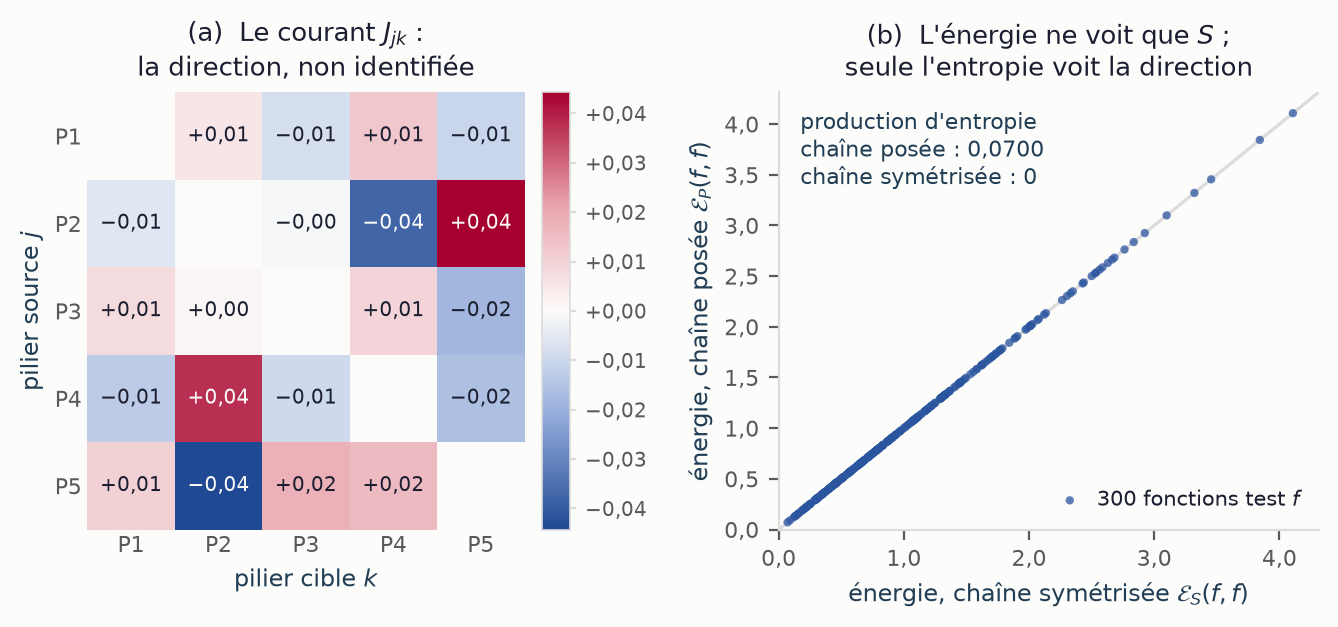
\includegraphics[width=0.95\textwidth]{Z11_reversibilite_martingale.png}
\caption{Direction et réversibilité. (a)~Le courant $J_{jk}=\pi_jP_{jk}-\pi_kP_{kj}$ est non nul, donc
le modèle a une direction. (b)~Pour trois cents fonctions test tirées au hasard, l'énergie de
fluctuation est la même pour la chaîne posée et pour sa symétrisée. La production d'entropie, mesure de dissymétrie des flux pondérés par leurs log-rapports, distingue ici les deux chaînes ; elle est nulle pour une chaîne réversible.}
\label{fig:reversibilite-rapport}
\end{figure}
% SOURCES-SCRIPTS: 40

\section{Expérience naturelle du choc MOVEit}

En mai 2023, l'exploitation de masse de la faille du logiciel de transfert MOVEit frappe en même
temps des centaines d'organisations. Si la contagion dirigée existe, ce choc exogène, daté et rattaché
au pilier~4, doit élever dans les mois suivants, chez les organisations touchées, le risque de
défaillances relevant d'autres piliers. Une différence de différences sur
188 organisations financières touchées, contre un groupe de contrôle apparié et sur des fenêtres de
$180$~jours, donne $+1{,}17$ jour de déclaration d'incident par organisation (IC bootstrap $[+1{,}07\,;+1{,}27]$).

Calé sur une fausse date un an plus tôt, le même dispositif donne $+1{,}11$. L'effet est donc
compatible avec une régression vers la moyenne du groupe de contrôle sélectionné, et l'effet net de $+0{,}06$ est
indiscernable de zéro. La cible resterait de toute façon non attribuable, car la source classe les
incidents par vecteur d'attaque, avec $32\,\%$ de non déterminés.

% SOURCES-SCRIPTS: 62 35

\section{Corpus de rapports post-incident}
\label{sec:postmortems}

Un rapport post-incident officiel reconstitue la séquence des défaillances de contrôle, ce
qu'aucune base agrégée ne fait. Nous codons sept rapports (Cyber Safety Review Board, FCA et PRA,
GAO, SEC, OCC), dont deux sur des entités financières régulées, en transitions dirigées $j \to k$
telles que le rapport les décrit. L'unité de codage est le couple (incident, paire de piliers).

Sur $17$ transitions, l'asymétrie $\Delta$ de l'équation~\eqref{eq:asymetrie} vaut $17$, contre $8{,}4 \pm 2{,}2$ sous un placebo par
permutation, d'où $z=+3{,}93$ ($p=0{,}0004$), là où le pas annuel d'OpRisk donnait $z=-0{,}33$.
Toutes les transitions vont dans le sens dominant de leur paire. P1, la gouvernance, n'est jamais une
cible ($9$ sorties, $0$ entrée) et P2, la gestion des incidents, n'a aucune sortie ($0$ sortie,
$7$ entrées), structure que le classeur qualitatif (la matrice $W$ posée à dire d'expert) posait par jugement.

Le placebo teste la cohérence du codage, mais pas l'exogénéité de la direction. Une enquête
officielle, mandatée pour déterminer une cause racine, conclut en effet souvent à une défaillance de
gouvernance, si bien que P1 peut ressortir comme source par convention d'écriture. S'y ajoutent un
codeur unique, des sources en partie secondaires et un échantillon d'incidents notoires. Le corpus
corrobore donc la structure sans la calibrer, et le coût du biais est borné au
\S\ref{sec:biais-narration}. Une mesure de fiabilité par second codeur en aveugle reste en attente.

Les trois relectures de praticiens reçues ne distinguent pas un ordre de propagation d'une cause
commune, ce qui corrobore la frontière mais pas la matrice. Les deux dernières contestent le sens
unique de deux arcs sans déplacer le capital publié (annexe~\ref{ch:elicitation}, \S\ref{sec:relecture-praticien}).
% SOURCES-SCRIPTS: 53

\section{Corpus étendu et matrice ordonnée}
\label{sec:corpus-etendu}

Nous ajoutons les trois rapports d'enquête publique sur CrowdStrike Falcon 2024, Log4Shell
2021--2022 et Raphaels Bank 2015. Le corpus compte alors $22$ transitions et le signal se renforce, y
compris lorsque l'on se restreint aux sources primaires ou à la perspective de l'entité.

\begin{center}\small
\renewcommand{\arraystretch}{1.25}
\begin{tabular}{@{}l r r r r@{}}
\toprule
\textbf{Périmètre} & \textbf{Rapports} & \textbf{Transitions} & \textbf{Asym.\ / nul} & $z$ \\
\midrule
Corpus initial (chapitre, ci-dessus) & $7$ & $17$ & $17$ / $8{,}4\pm2{,}2$ & $+3{,}93$ \\
\textbf{Corpus étendu} & $10$ & $22$ & $22$ / $9{,}5\pm2{,}4$ & $\mathbf{+5{,}12}$ \\
Sources \emph{primaires} seules & $7$ & $18$ & $18$ / $8{,}2\pm2{,}4$ & $+4{,}08$ \\
Perspective \emph{entité} seule & $6$ & $16$ & $16$ / $8{,}0\pm2{,}2$ & $+3{,}62$ \\
\bottomrule
\end{tabular}
\end{center}

\vspace{2pt}
\noindent Chaque incident déclare aussi l'ensemble des piliers défaillants, y compris ceux qui n'ont
rien entraîné. On en tire le dénominateur manquant et la matrice ordonnée complète :
\begin{equation}
\begin{gathered}
  p_{jk} \;=\; \Prob(\text{le rapport documente } j\to k \mid \text{le pilier } j \text{ a cédé}),
  \\
  p_{jk}\mid\text{données} \;\sim\; \mathrm{Beta}\bigl(1+m_{jk},\;1+N_j-m_{jk}\bigr),
\end{gathered}
  \label{eq:pjk}
\end{equation}
où $N_j$ compte les incidents où $j$ a cédé et $m_{jk}$ ceux où le rapport documente $j\to k$,
sous un a priori uniforme. Sur les
vingt liens ordonnés, douze ont un intervalle de crédibilité à $90\,\%$ situé sous $0{,}5$ et aucun au-dessus, si bien
que les transitions documentées y sont rares sans identifier les propagations fortes. Les liens les plus élevés,
$P_3\to P_2$ ($0{,}77$, intervalle $[0{,}48\,;0{,}95]$) et $P_1\to P_4$ ($0{,}68$, $[0{,}40\,;0{,}89]$),
recouvrent encore $0{,}5$.

Les douze liens faibles comprennent les quatre sorties de $P_2$ et trois des quatre entrées de $P_1$,
l'arc $P_5 \to P_1$ n'étant pas classé faible. La corrélation avec le classeur d'expert n'est pas
significative ($\rho=+0{,}08$ sur la matrice, $+0{,}31$ sur sa partie antisymétrique, $p=0{,}19$).
Si l'on ajoute au dénominateur des défaillances non propagées, le niveau moyen de $p_{jk}$ tombe de
$0{,}27$ à $0{,}07$, mais la part de direction $\lVert A\rVert/\lVert W\rVert$ reste à $60\,\%$.
Ce postérieur porte sur la documentation des transitions dans le corpus sélectionné ; l'absence de mention ne prouve pas l'absence de propagation. Le corpus suggère un ordre, sans en fixer l'intensité.
% SOURCES-SCRIPTS: 59

\section{Biais de narration}
\label{sec:biais-narration}

Onze des vingt-deux transitions codées partent de $P_1$, ce qu'une convention de cause racine pourrait
produire. Nous chiffrons ce biais par une loi nulle exacte, obtenue par convolution, et par une borne
adverse sur les $2^{11}$ sous-ensembles d'arêtes partant de $P_1$. Le jackknife retire successivement
chaque rapport ; le signal ne tient pas à un rapport isolé.

\begin{center}\small
\renewcommand{\arraystretch}{1.25}
\begin{tabular}{@{}l l l@{}}
\toprule
\textbf{Hypothèse sur les $11$ arêtes de $P_1$} & \textbf{Reste} & $p$ \textbf{exacte} \\
\midrule
Aucune (corpus tel qu'il est codé) & $22$ transitions & $1{,}5\cdot10^{-5}$ \\
$4$ arêtes \emph{retournées}, pire configuration & $22$ transitions & $\mathbf{0{,}084}$ \\
Les $11$ arêtes \emph{retirées} & $11$ transitions & $0{,}0039$ \\
Les $7$ \emph{rapports} concernés retirés & $3$ transitions & $0{,}50$ \\
\bottomrule
\end{tabular}
\end{center}

\vspace{2pt}
\noindent Il faudrait que la convention narrative ait inversé quatre des onze arêtes, dans
l'agencement le plus défavorable, pour perdre la significativité. Retirer tout le rôle de la
gouvernance, la moitié du corpus, ne suffit pas, car la direction subsiste dans les chaînes
$P_3\to P_2$ et $P_4\to P_2$, où $P_1$ ne figure pas. Retirer les sept rapports entiers écarte aussi
des chaînes que le biais ne concerne pas.

En capital, nous dégradons l'émission de $P_1$ par $W_{1k}\to(1-a)\,W_{1k}$ et recalculons la bande
à chaque degré, avec la cascade indépendante des calculs d'entité. Le besoin extrapolé de l'entité notionnelle (\S\ref{sec:entites-reelles}) passe de $24{,}1$ à
$15{,}0$~M\euro{} lorsque les transmissions depuis $P_1$ sont annulées ($-37{,}7\,\%$). Ce déplacement de $9{,}1$~M\euro{} représente
$0{,}78$ fois la largeur de la bande d'identification, $11{,}7$~M\euro, de sorte qu'admettre
l'objection dans toute son ampleur coûte moins que l'ignorance directionnelle déjà publiée. Le pilier
à remédier en premier passe toutefois de $P_1$ à $P_4$ dès $a = 0{,}50$. L'écart entre états de
conformité descend de $+83{,}0\,\%$ à $a=0$ à $+40{,}6\,\%$ à $a=1$ sans s'annuler, car la
conformité agit par $g$ sur toutes les arêtes.

% SOURCES-SCRIPTS: 54
% SOURCES-SCRIPTS: 64 65 136

\section{Formalisation bayésienne}
\label{sec:bayes}

Nous exploitons le même matériau dans un cadre bayésien, en posant un lien, que la donnée ne permet pas de vérifier, entre la fréquence d'une chaîne dans les rapports et le sens de la propagation. Pour chaque paire
$\{lo,hi\}$ de piliers, on note $\theta$ la probabilité qu'une chaîne documentée aille de $lo$ vers $hi$,
reliée au coefficient antisymétrique par
\[
  A_{lo,hi} \;=\; S_{lo,hi}\,(2\theta - 1),
\]
bijection croissante de $[0,1]$ sur l'intervalle admissible $[-S_{lo,hi},+S_{lo,hi}]$ du
chapitre~\ref{chap:partielle}. Les indices $lo$ et $hi$ désignent les deux piliers par indice croissant.
Les paramètres $\alpha_0,\beta_0$ règlent l'a priori ; $\mathcal{B}\mathrm{in}$ est la loi binomiale
des comptages de sens. Avec $n_{lo}$ chaînes de $lo$ vers $hi$ et $n_{hi}$ dans l'autre sens,
\begin{equation}
  \begin{gathered}
  \theta \sim \mathrm{Beta}(\alpha_0,\beta_0),
  \qquad
  n_{lo}\mid\theta \sim \mathcal{B}\mathrm{in}(n_{lo}+n_{hi},\,\theta)
  \\
  \Longrightarrow\qquad
  \theta \mid \text{données} \;\sim\; \mathrm{Beta}\bigl(\alpha_0+n_{lo},\;\beta_0+n_{hi}\bigr).
  \end{gathered}
  \label{eq:posterieur-beta}
\end{equation}
Les quatre paires que le corpus ne documente pas gardent sous $\mathrm{Beta}(1,1)$ un $\theta$
uniforme, donc un coefficient qui couvre tout l'intervalle admissible. Le postérieur reproduit
l'identification partielle sans la poser. Le capital devient une loi, dont l'intervalle de
crédibilité à $90\,\%$ est $81\,\%$ plus resserré que les bornes de pire cas
(bornes du chapitre~\ref{chap:partielle}). Sous un prior sceptique, la médiane bouge à peine, mais seules deux des six
paires documentées ont un intervalle de crédibilité à $90\,\%$ qui exclut $\theta=1/2$. Nous retenons les bornes et publions l'intervalle à titre informatif.
% SOURCES-SCRIPTS: 56

\section{Frontière d'identification}

\begin{center}\small
\renewcommand{\arraystretch}{1.3}
\begin{tabular}{@{}p{3.2cm} p{7.4cm} p{4.2cm}@{}}
\toprule
\textbf{Objet} & \textbf{Ce que la donnée établit} & \textbf{Posture retenue} \\
\midrule
\textbf{Structure} \newline (P1 amont, P2 aval) &
$17$ transitions sur le corpus initial et $22$ sur le corpus étendu, aucune à contre-sens,
$z=+3{,}9$ puis $+5{,}1$ ; accord de la structure avec le classeur d'expert, non des coefficients ($\rho=+0{,}08$) ; codeur unique &
\textbf{revendiquée}, avec son confondant déclaré \\
\textbf{Direction} \newline paire par paire &
$2$ paires sur $6$ seulement ont un intervalle de crédibilité concluant &
\textbf{non revendiquée} ; les bornes restent \\
\textbf{Amplitude} \newline des coefficients &
aucune information ; même les dix sens connus, une bande de $656$~M\euro{} subsisterait &
\textbf{non identifiable} par cette voie \\
\bottomrule
\end{tabular}
\end{center}

\vspace{4pt}
\noindent Le corpus ne calibre pas $W$. Le chapitre~\ref{chap:partielle} explore les directions,
puis la section~\ref{ch:livrable} chiffre l'intérêt conditionnel d'un registre.

% SOURCES-SCRIPTS: 55 59 64
